% !TEX encoding = UTF-8 Unicode
\documentclass[a4paper]{article}

\usepackage{color}
\usepackage{url}
\usepackage[T2A]{fontenc} % enable Cyrillic fonts
\usepackage[utf8]{inputenc} % make weird characters work
\usepackage{graphicx}

\usepackage[english,serbian]{babel}
%\usepackage[english,serbianc]{babel} %ukljuciti babel sa ovim opcijama, umesto gornjim, ukoliko se koristi cirilica

\usepackage[unicode]{hyperref}
\hypersetup{colorlinks,citecolor=green,filecolor=green,linkcolor=blue,urlcolor=blue}

\usepackage{listings}

\usepackage{booktabs} 

%\newtheorem{primer}{Пример}[section] %ćirilični primer
\newtheorem{primer}{Primer}[section]

\definecolor{mygreen}{rgb}{0,0.6,0}
\definecolor{mygray}{rgb}{0.5,0.5,0.5}
\definecolor{mymauve}{rgb}{0.58,0,0.82}

\lstset{ 
  backgroundcolor=\color{white},   % choose the background color; you must add \usepackage{color} or \usepackage{xcolor}; should come as last argument
  basicstyle=\scriptsize\ttfamily,        % the size of the fonts that are used for the code
  breakatwhitespace=false,         % sets if automatic breaks should only happen at whitespace
  breaklines=true,                 % sets automatic line breaking
  captionpos=b,                    % sets the caption-position to bottom
  commentstyle=\color{mygreen},    % comment style
  deletekeywords={...},            % if you want to delete keywords from the given language
  escapeinside={\%*}{*)},          % if you want to add LaTeX within your code
  extendedchars=true,              % lets you use non-ASCII characters; for 8-bits encodings only, does not work with UTF-8
  firstnumber=1000,                % start line enumeration with line 1000
  frame=single,	                   % adds a frame around the code
  keepspaces=true,                 % keeps spaces in text, useful for keeping indentation of code (possibly needs columns=flexible)
  keywordstyle=\color{blue},       % keyword style
  language=Python,                 % the language of the code
  morekeywords={*,...},            % if you want to add more keywords to the set
  numbers=left,                    % where to put the line-numbers; possible values are (none, left, right)
  numbersep=5pt,                   % how far the line-numbers are from the code
  numberstyle=\tiny\color{mygray}, % the style that is used for the line-numbers
  rulecolor=\color{black},         % if not set, the frame-color may be changed on line-breaks within not-black text (e.g. comments (green here))
  showspaces=false,                % show spaces everywhere adding particular underscores; it overrides 'showstringspaces'
  showstringspaces=false,          % underline spaces within strings only
  showtabs=false,                  % show tabs within strings adding particular underscores
  stepnumber=2,                    % the step between two line-numbers. If it's 1, each line will be numbered
  stringstyle=\color{mymauve},     % string literal style
  tabsize=2,	                   % sets default tabsize to 2 spaces
  title=\lstname                   % show the filename of files included with \lstinputlisting; also try caption instead of title
}

\begin{document}

\title{Šta čini univerzitetski kurs teškim?\\ \small{Seminarski rad u okviru kursa\\Metodologija stručnog i naučnog rada\\ Matematički fakultet}}

\author{
    \makebox[\linewidth][c]{Jovan Vukićević, Jovan Škorić, Nikola Kuburović, Radenko Nikolić} \\ 
    \makebox[\linewidth][c]{jovanvukicevic@hotmail.com, jovanskoric02@gmail.com,} \\
    \makebox[\linewidth][c]{nikola.kuburovic123@gmail.com, radenko.nikolic01@gmail.com}
}

%\date{9.~april 2015.}

\maketitle

\abstract{
Teški univerzitetski kursevi predstavljaju jednu od glavnih prepreka pri studentovom prolasku kroz studije. U ovom radu istražujemo različite faktore organizacije kurseva koji utiču na njihovu težinu, počev od aspekata organizacije nastave do aspekata organizacije ispita. Na kraju rada prikazujemo rezultate ankete sprovedene nad studentima Matematičkog fakulteta Univerziteta u Beogradu i predstavljamo njihova lična iskustva sa teškim univerzitetskim kursevima, kao i upoređujemo dobijene zaključke sa zaključcima u literaturi.
}

\tableofcontents

\newpage

\section{Uvod}
\label{sec:uvod}

Srž studija na univerzitetu čine univerzitetski kursevi. Samim tim, težinu studija možemo poistovetiti sa težinom kurseva na njima. Iako se u osnovi težine univerzitetskog kursa nalaze kompleksnost same oblasti koja se obrađuje i količina studentskog predznanja, postoje razni drugi faktori koji doprinose težini kursa.

Glavni cilj univerzitetskih profesora je da prenesu znanje studentima na što efikasniji način, što podrazumeva jednostavnost u prenošenju iskustava u razumevanju problema. U odnosu na nastavnike na prethodnim obrazovnim nivoima, univerzitetski profesori imaju mnogo veću slobodu u dizajniranju kurseva koje predaju. Podešavanjem raznih aspekata tih kurseva, oni direktno utiču na njegovu težinu.

Kao pomoć profesorima u dizajniranju svojih kurseva, kao i uvid u šta to čini univerzitetski kurs teškim, u ovom radu ćemo prikazati osnovne karakteristike teških univerzitetskih kurseva, kao i dati predloge kako ih načiniti lakšim. Zarad ovog cilja, sproveli smo i anketu nad studentima Matematičkog fakulteta Univerziteta u Beogradu, čiji rezultat ćemo prezentovati u ovom radu.

\section{Organizacija nastave}
Organizacija nastave ima ključnu ulogu u oblikovanju univerzitetskog iskustva studenata i
značajno utiče na percepciju težine kursa. Na osnovu dostupne literature, nekoliko ključnih
faktora doprinosi efektivnoj organizaciji nastave: jasno definisani ishodi učenja, pažljivo
strukturisanje sadržaja, odgovarajući tempo predavanja, primena praktičnih primera u
nastavi i online nastava.

\subsection{Ishodi učenja i planiranje nastave}
Jasno definisani ishodi učenja čine osnovu uspešne organizacije nastave. Ishodi moraju biti
usklađeni s industrijskim standardima i realnim potrebama tržišta rada kako bi studenti mogli
da povežu teorijsko znanje sa praktičnim zahtevima profesije. Teorija konstruktivne
usklađenosti (slika \ref{fig:konstruktivna_uskladjenost}), koju su predložili Biggs i Tang \cite{biggs2007teaching}, naglašava da ishodi učenja, nastavne
aktivnosti i ocenjivanje treba da budu međusobno povezani kako bi se maksimizovala
efikasnost obrazovnog procesa. Ova usklađenost ne samo da poboljšava razumevanje, već i
smanjuje osećaj zbunjenosti kod studenata, što direktno utiče na percepciju težine kursa.

Literatura takođe ističe potrebu za dubinskim pokrivanjem osnovnih koncepata, umesto
pokušaja da se obuhvati širok spektar tema bez dovoljno objašnjenja. Kane, Rockoff i
Staiger \cite{kane2006certification} navode da prevelika količina gradiva, koja nije jasno povezana s praktičnim
primerima, često dovodi do pada akademskih postignuća studenata. Slično tome, Smith
\cite{smith2009simulation} ističe da neuspeh u naglašavanju osnovnih veština i znanja utiče na percepciju kursa
kao teškog. Osnovno pravilo je da kurs treba da bude prilagođen razumevanju
studenata, s progresivnim uvodom u složenije teme kako bi se omogućio postepen prelazak
na naprednije koncepte.

Učestali problemi s organizacijom nastave uključuju dodavanje suvišnih ili nepotrebnih
tema u kurs, nedostatak jasnoće u vezi sa sekvenciranjem gradiva i neprilagođeno
vreme za pojedine teme. Na primer, istraživanja su pokazala da neadekvatno vremensko
planiranje za pojedine aspekte gradiva često dovodi do osećaja preopterećenja kod
studenata.

\begin{figure}[h!]
\begin{center}
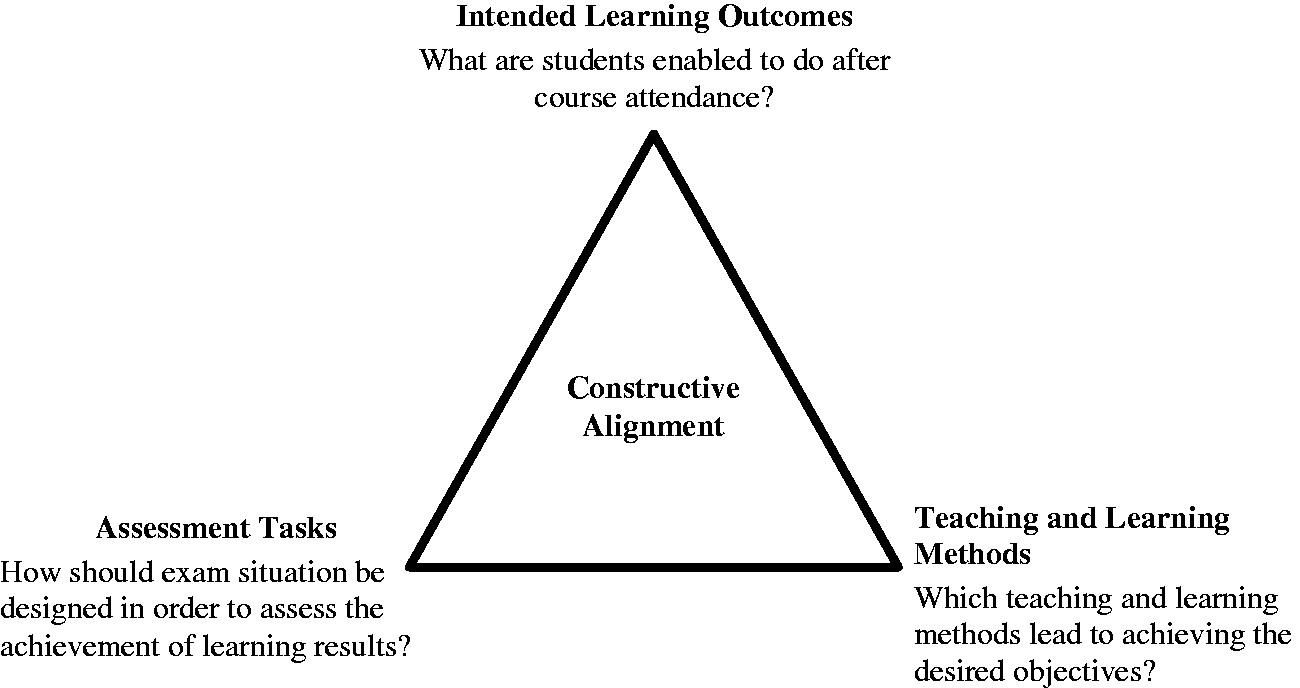
\includegraphics[scale=2]{constructive_alignment.jpeg}
\end{center}
\caption{Konstruktivna usklađenost}
\label{fig:konstruktivna_uskladjenost}
\end{figure}

\subsection{Tempo izvođenja nastave}
Tempo nastave značajno utiče na percepciju težine kursa i na sposobnost studenata da
razumeju i savladaju gradivo. Brza predavanja, koja ne ostavljaju prostor za diskusiju i
dodatna objašnjenja, mogu povećati osećaj frustracije kod studenata. Prema istraživanjima,
loše tempirana nastava često ostavlja studente s nedovoljno vremena za procesuiranje
informacija, što negativno utiče na rezultate ispita i percepciju kursa.

Daka \cite{daka2020exploration} navodi da je pažljivo planiranje nastavnih aktivnosti ključno za uspešnu
nastavu. Uključivanje raznovrsnih nastavnih metoda, kao što su praktične vežbe, grupni rad i
studije slučaja, doprinosi dubljem razumevanju gradiva i povećava angažovanost studenata.
Changwe i saradnici \cite{daka2020exploration} sugerišu da predavači treba da izbegavaju prebrzo prelazak s
jedne teme na drugu, jer to može izazvati zbunjenost i otežati praćenje nastave.
Još jedan važan aspekt tempa nastave je korišćenje jasno definisanih prelaza između
različitih delova predavanja. Na primer, jasno razdvajanje tema i objašnjenja omogućava
studentima da prepoznaju ključne tačke predavanja, što dodatno pomaže u zadržavanju
pažnje i razumevanju kompleksnih tema. Pored toga, postavljanje logičnog toka gradiva, gde
se složene teme nadovezuju na osnovne koncepte, značajno doprinosi smanjenju osećaja
preopterećenja.

\subsection{Relevantnost sadržaja}
Sadržaj kursa mora biti jasno povezan sa stvarnim aplikacijama i profesionalnim zahtevima,
jer to povećava motivaciju i angažovanost studenata. Predavanja koja uspešno povezuju
teorijske koncepte s praktičnim primerima omogućavaju studentima da bolje razumeju kako
se stečeno znanje primenjuje u praksi. Sarfraz i saradnici \cite{sarfraz2022viability} navode da je kombinacija
tradicionalne nastave i tehnologije, kao što je kombinovano učenje (eng.~{\em blended learning}, slika \ref{fig:kombinovano_ucenje}), posebno korisna za studente
jer omogućava fleksibilniji pristup učenju i bolju primenu gradiva.

Problemi nastaju kada kursevi sadrže previše zastarelih ili nerelevantnih tema. Na primer,
ako predavanja uključuju koncepte koji više nisu primenljivi u modernim profesionalnim
okruženjima, studenti gube interes i kurs se doživljava kao suvišno težak. Na osnovu
istraživanja, prilagođavanje sadržaja savremenim industrijskim standardima i kontinuirano
preispitivanje kursa ključno je za rešavanje ovih problema.

\begin{figure}[h!]
\begin{center}
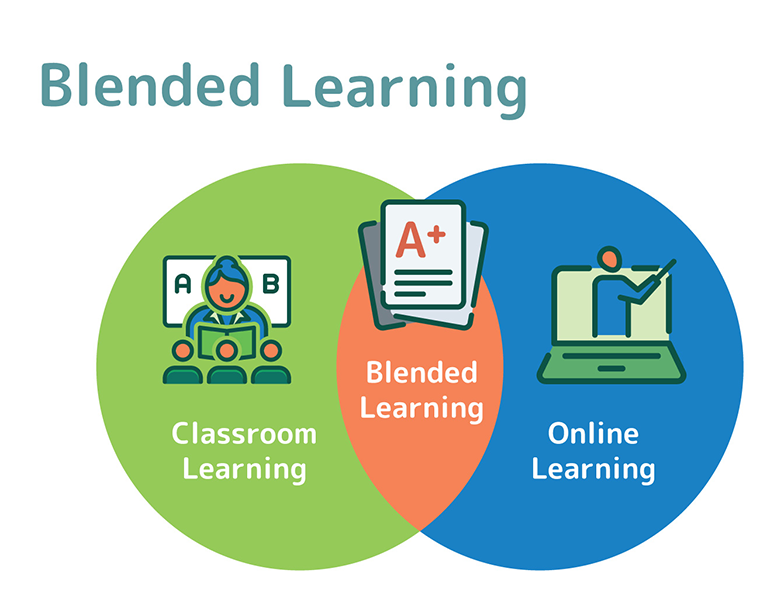
\includegraphics[scale=0.4]{blended_learning.png}
\end{center}
\caption{Kombinovano učenje}
\label{fig:kombinovano_ucenje}
\end{figure}

\subsection{Online nastava i njeni izazovi}

Pandemija je, pored ozbiljnih promena na globalnom nivou, donela i promenu u načinu odvijanja nastave, primoravajući obrazovne institucije da pređu na online režim rada. Iako je u mnogim aspektima ovaj prelazak olakšao studiranje, izazvao je i brojna otežanja pri polaganju ispita za mnoge studente.

Prelazak na online nastavu doveo je do smanjenja direktne komunikacije između profesora i studenata, što je od suštinskog značaja za proces učenja. Gamage i saradnici \cite{gamage2022rethinking} ističu da je smanjenje interakcije povećalo osećaj izolovanosti kod studenata i negativno uticalo na kvalitet obrazovanja, jer su se mnogi nastavnici oslanjali na tradicionalne metode predavanja bez adekvatne adaptacije digitalnom formatu.

Dodatni problem predstavlja nedostatak opreme, koji je često uzrokovan finansijskim poteškoćama, što je mnoge studente dovelo u nepovoljan položaj. Kvalitet prenosa znanja varirao je od predmeta do predmeta, jer neki profesori nisu bili dovoljno pripremljeni za prelazak na online režim nastave. Zbog toga su se studenti često oslanjali na samostalno učenje i traženje dodatnih informacija.

Takođe, online režim nastave uneo je mnogim studentima dodatnu nesigurnost, posebno u pogledu njihovog znanja, zbog otežane komunikacije sa profesorima, smanjene mogućnosti za postavljanje pitanja i dobijanje povratnih informacija, kao i smanjene razmene iskustava među studentima, što je dodatno povećalo nivo stresa prilikom pripreme i samog polaganja ispita.

\vspace{8mm}

Ovi elementi organizacije nastave ključni su za oblikovanje akademskog iskustva studenata.
Pažljivo osmišljeni kursevi, sa jasno definisanim ciljevima i odgovarajućim tempom, ne samo
da smanjuju percepciju težine kursa, već i obezbeđuju kvalitetnije obrazovanje i bolje
rezultate.

\section{Organizacija ispita}

Polaganje ispita je oduvek bilo značajan izazov za studente, ali savremeno obrazovanje donelo je dodatne faktore koji mogu otežati ovaj proces.


\subsection{Nenadoknadivi kolokvijumi}

Kolokvijumi imaju ključnu ulogu u obrazovanju, jer omogućavaju studentima da kontinuirano prate svoje znanje i olakšavaju završnu pripremu za ispite. Međutim, uvođenjem koncepta nenadoknadivih kolokvijuma, često se pretvara u izvor nepotrebnog stresa i pritiska za studente. Sistemi koji ne omogućavaju prilagodljivost za nepredviđene okolnosti, kao što su bolest ili druge životne situacije, mogu dodatno ugroziti akademski uspeh.

Prema Gamage i saradnicima \cite{gamage2022rethinking}, fleksibilnost u sistemima ocenjivanja ključna je za stvaranje jednakih prilika za sve studente. U situacijama gde su zadaci nenadoknadivi, studenti suočeni s vanrednim okolnostima, poput bolesti, često su primorani da se oslanjaju isključivo na završni ispit, što povećava nivo stresa i otežava pripremu.

Carter i Hogan \cite{carter2013authentic} ukazuju na to da autentične metode ocenjivanja, koje omogućavaju prilagođavanje individualnim potrebama studenata, mogu smanjiti pritisak i podstaći aktivno učenje. Takve metode uključuju dodatne rokove ili alternativne zadatke za studente koji su opravdano izostali sa kolokvijuma, čime se povećava pravednost i motivacija za učenje.

Nenadoknadivi kolokvijumi često se negativno odražavaju i na sveukupno iskustvo studenata, jer ne uzimaju u obzir raznolikost njihovih situacija. Ova rigidnost može dovesti do toga da studenti izgube pravo na polaganje ispita u tekućoj školskoj godini, čak i u situacijama koje su van njihove kontrole. Ovakav pristup ne samo da povećava stres, već smanjuje i efikasnost obrazovnog procesa, što se može ublažiti uvođenjem fleksibilnijih i inkluzivnijih rešenja.

\subsection{Neravnoteža između težine ispita i gradiva sa nastave}

Jedan od čestih problema na koji studenti ukazuju jeste neravnoteža između težine zadataka na ispitima i primera obrađenih tokom predavanja i vežbi. Ovakva praksa može obeshrabriti studente, jer često imaju osećaj da materijali i primeri sa nastave nisu adekvatna priprema za ispit. Istraživanja ukazuju da ovakva razlika može biti rezultat pokušaja profesora da ocene sposobnost studenata za primenu znanja u novim i nepoznatim situacijama, ali se često pokazuje kao kontraproduktivna.

Studije pokazuju da studenti bolje usvajaju gradivo kada su ispiti u skladu s primerima iz nastave, jer to smanjuje nesigurnost i povećava motivaciju za učenje (\cite{sambell2013assessment}). Ova korelacija između zadataka sa časova i ispita omogućava studentima da bolje razumeju očekivanja i da razviju veštine neophodne za uspeh na ispitu. Prema Grahamu \cite{graham1999practice}, uključenje zadataka koji su slični ili povezani s predavanjima pomaže studentima da konsoliduju svoje znanje i razviju dublje razumevanje gradiva.

Razlike u težini između zadataka sa nastave i ispita često vode do povećanja stresa kod studenata i osećaja nepripremljenosti. Rešenja uključuju bolje usklađivanje nastavnih metoda s ciljevima ispita i transparentnu komunikaciju o očekivanjima profesora. Treba uzeti u obzir da prevelika sličnost između zadataka s predavanja i zadataka na ispitu može podstaći studente da nauče ispitno gradivo napamet, bez dubljeg razumevanja.

\subsection{Prezahtevno ocenjivanje}

Prestrogi kriterijumi ocenjivanja mogu značajno otežati polaganje ispita, jer studenti, umesto da se fokusiraju na razumevanje gradiva, često postaju preokupirani ispunjavanjem strogo definisanih i ponekad preteranih zahteva. Istraživanja pokazuju da jasno definisani standardi ocenjivanja i pružanje konstruktivnih povratnih informacija omogućavaju studentima da se fokusiraju na sadržaj i bolje razumeju gradivo, umesto da se previše usmere na tehničke aspekte ocenjivanja (\cite{gamage2022rethinking}). 

Ovaj pristup može povećati poverenje studenata u proces i učiniti ga manje stresnim, što doprinosi boljoj efikasnosti u učenju.

Treba uzeti u obzir da prevelika sličnost izmedju zadataka sa predavanja i zadataka na ispitu može podstaći studente da nauče ispitno gradivo napamet, bez
dubljeg razumevanja.

\subsection{Odnos usmene i pismene provere znanja}

Razlika između usmenih i pismenih ispita je očigledna, jer svaki od njih nosi svoje prednosti i izazove. Pismeni ispiti pružaju veću objektivnost, jer su pitanja ista za sve studente, a uslovi pod kojima se polažu ispit su jednaki za sve. Ovaj pristup omogućava profesorima da ocene znanje studenata na standardizovan način, smanjujući mogućnost subjektivnosti. S druge strane, usmeni ispiti omogućavaju profesorima da se bolje upoznaju s razumevanjem studenta i da prilagode pitanja ili pristup u skladu sa studentovim znanjem i reakcijama. Iako ovo može pružiti dublju procenu, usmeni ispiti često izazivaju dodatni stres kod studenata. Mnogi se suočavaju s teškoćama u verbalnom izražavanju svojih misli u kratkom vremenskom intervalu, dok su neki pod pritiskom zbog toga što je profesor usmerio svoju pažnju isključivo na njih. Pismeni ispiti, s druge strane, omogućavaju studentima da imaju više vremena da razmisle, formulišu odgovore i preciznije predstave svoje znanje, ali postoji rizik da zadaci budu previše zahtevni i da se ne odražavaju uvek adekvatno na sposobnosti studenata. Prema istraživanjima, usmeni ispiti omogućavaju fleksibilniji pristup i mogu otkriti dublje razumevanje, ali su često stresniji za studente (\cite{huxham2010oral}). Pismeni ispiti, iako manje stresni, ponekad ne omogućavaju toliku dubinsku procenu razumevanja kao usmeni ispiti.

\subsection{Podela ispita na delove i završni ispit}

Podela ispita u manje, tematski povezane segmente omogućava studentima da se fokusiraju na specifične oblasti gradiva, čime se smanjuje stres jer ne moraju da se pripremaju za jedan veliki ispit. Ovakav pristup omogućava bolje praćenje napretka studenata, jer se vrednuje znanje u manjim, lakšim za savladavanje celinama. Međutim, previše delova može postati problematično, jer se od studenata očekuje da savladaju previše materijala u kratkom vremenu. Dodatno, kada se u okviru sistema ocenjivanja pojavi i završni ispit koji pokriva sve oblasti gradiva, studenti mogu biti pod dodatnim stresom jer moraju da integrišu sve naučeno u jednoj poslednjoj proceni.

Previše ispita tokom semestra, zajedno sa obavezom završnog ispita, može povećati pritisak na studente, naročito ako svaki deo zahteva duboko razumevanje gradiva i precizno razmišljanje. Graham \cite{graham1999practice} ukazuje da učestali ispiti mogu smanjiti efikasnost učenja, dok Tuckman \cite{tuckman1998benefits} naglašava da bi trebalo balansirati broj testova kako bi se smanjilo preopterećenje. Kombinacija manjih testova i jednog sveobuhvatnog završnog ispita može omogućiti studentima da pokažu svoje celokupno razumevanje gradiva, a da pri tome ne budu previše opterećeni.

\section{Rezultati ankete}

U odgovaranju na pitanja iz ankete učestvovao je 61 student
Matematičkog fakulteta u Beogradu, sa različitih stepena studija (slika \ref{fig:stepen_studija}).

\begin{figure}[h!]
\begin{center}
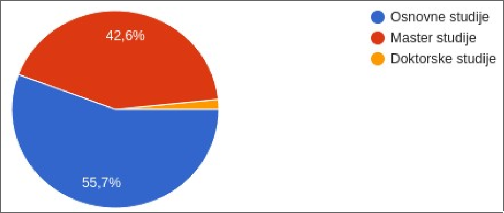
\includegraphics[scale=0.35]{stepen_studija_pie.png}
\end{center}
\caption{Raspodela studenata prema stepenu studija}
\label{fig:stepen_studija}
\end{figure}

Većina ispitanika (77\%) smatra da su matematički kursevi teži od informatičkih, što može biti rezultat složenosti gradiva i visoke apstraktnosti koja je karakteristična za matematičke predmete. Ispitanici koji su odgovarali na pitanje o najtežim delovima kursa najviše su se složili da su teorijski ispiti najveći izazov, posebno kada je u pitanju ogromna količina složenih i međusobno povezanih teorijskih pojmova koji se moraju savladati za polaganje. Na osnovu komentara, evidentno je da studenti smatraju da je visoka apstraktnost i apstraktno razmišljanje u matematici nešto što čini ove kurseve izazovnijim od informatičkih.

Iz odgovora na pitanje o najtežim kursevima, primećuje se da su najčešće pominjani predmeti Verovatnoća, Analiza 1 i Analiza 2. Ovo potvrđuje prethodne odgovore u kojima studenti ističu ove kurseve kao najzahtevnije zbog obimnog i kompleksnog gradiva. U komentaru koji je pratila Analiza 1, studenti su naglasili da je kurs veoma težak za početnike jer se uvode potpuno nove definicije i teorije koje studentima nisu intuitivne, a zatim se traži duboko razumevanje teorije i sposobnost primene u praktičnim zadacima. Ovo stvara značajan izazov, jer studenti često nisu u mogućnosti da pravilno usvoje gradivo bez jasnog objašnjenja i vežbi koje će im omogućiti da se pripreme za složene ispite.

Jedan od glavnih izazova koji su studenti istakli je i pretežak usmeni ispit, posebno za kurs Verovatnoće, koji mnogi smatraju nekorektno organizovanim. Usmeni ispit se često doživljava kao veoma stresan jer se od studenata očekuje vrlo visok nivo teorijskog znanja, dok se u nekim slučajevima smatra da predavači nisu pružili dovoljno konkretnih i jasnih uputstava o tome šta tačno treba da znaju studenti. Takođe, ponekad se dešava da se ispituju teme koje nisu bile adekvatno obrađene na predavanjima, što dodatno frustrira studente. Ovo ukazuje na potrebu za bolje definisanim smernicama kada je u pitanju usmeni ispit, kao i za većom povezanošću teorijskog znanja sa zadacima na ispitima.

Analiza 2 je još jedan predmet koji se često spominje kao izuzetno težak, zbog velikog obima gradiva koje je potrebno savladati, ali i nedostatka jasnoće u literaturi koja se koristi za učenje. Studenti su se žalili na obiman materijal, ali i na to da vežbe nisu u dovoljnoj meri pratile težinu ispita. Pored toga, studenti su naglasili da se predavanja često ne usklađuju sa zahtevima ispita, što stvara poteškoće u pripremi, jer nisu sigurni koji delovi gradiva su zaista ključni. Neki su komentarisali da je potrebno uložiti više truda u jasno objašnjavanje teorije koja se koristi u nastavku studija, jer mnogi smatraju da im nije dovoljno jasno kako će primeniti naučeno na budućim kursevima.

Jedan od često ponavljanih problema je i neprilagođenost usmenih ispita za studente sa informacijama sa smera Informatika, jer im se ponekad čini da su ispitni zahtevi više usmereni na teoriju verovatnoće nego na primenu matematike u informatičkim problemima. Ovo ukazuje na potrebu za većom specijalizacijom ispita i gradiva, kako bi se studentima sa različitim interesovanjima i usmerenjima omogućila bolja priprema i veće razumevanje materijala.

Kada su u pitanju praktični problemi u vezi sa organizacijom ispita, studenti su takođe istakli da postoji određena neprilagođenost kada su u pitanju zadaci na pismenim ispitima. Iako su neki studenti smatrali da su zadaci ponekad previše kompleksni ili nemogući da se reše u vremenskom okviru, mnogi su komentarisali da se na ispitu pojavljuju zadaci koji nisu bili adekvatno vežbani na predavanjima. Studenti su stoga predložili da bi trebalo uvesti više vežbi sa zadacima koji su slični onima koji će se pojaviti na ispitu, čime bi se omogućilo studentima da se bolje pripreme i steknu sigurnost u svoje znanje. Takođe, povećanje broja dostupnih materijala za učenje i vežbanje bila je još jedna sugestija koja bi mogla doprineti boljoj pripremi i manjoj stresnosti ispita.

Osim toga, studenti su se osvrnuli na nedostatak interakcije sa profesorima i asistentima tokom nastave i vežbi (slika \ref{fig:nedostatak_interakcije}).

\begin{figure}[h!]
\begin{center}
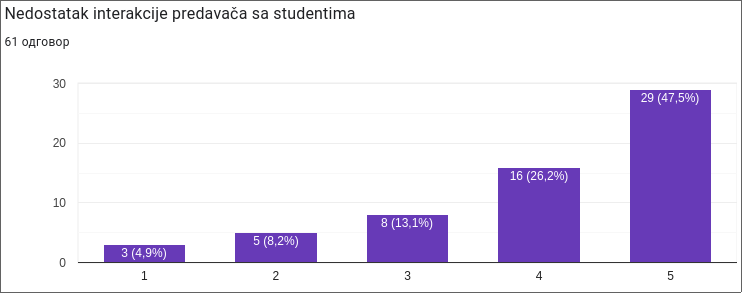
\includegraphics[scale=0.37]{nedostatak_interakcije.png}
\end{center}
\caption{Uticaj nedostatka interakcije predavača sa studentima}
\label{fig:nedostatak_interakcije}
\end{figure}

Veći broj komentara je ukazao na to da nedostatak redovnih povratnih informacija o napretku studenata može uticati na njihov osećaj sigurnosti u gradivu. Studenti smatraju da je važno imati jasne smernice i mogućnost za konsultacije sa profesorima, kao i redovno dobijanje povratnih informacija, kako bi mogli da poboljšaju svoje razumevanje gradiva i pravilno se pripreme za ispite.

Pored ovih izazova, studenti su predložili i rešenja koja se mogu implementirati kako bi se olakšala priprema za ispite. Najčešće predloženo rešenje bilo je razdvajanje težih kurseva na manje delove, odnosno uvođenje predispitnih obaveza, čime bi se studentima omogućilo da lakše savladaju gradivo kroz manje, ali konkretne korake. Takođe, smanjenje obima gradiva i usmeravanje na ključne teme takođe bi značajno olakšalo studijama, jer studenti smatraju da trenutno moraju savladati previše gradiva koje nije uvek jasno povezano sa stvarnim potrebama i izazovima na ispitima.

Iako je online nastava bila spomenuta kao potencijalni problem, samo 29.6\% ispitanika smatra da je ona otežala kurs, dok ostali smatraju da nije uticala ni pozitivno ni negativno. Ovaj rezultat ukazuje na to da nisu svi studenti imali isto iskustvo sa online nastavam, te se može pretpostaviti da je kvaliteta nastave i interakcije sa profesorima tokom online nastave varirala.

Na kraju, zaključujemo da su Verovatnoća i Analize 1 i 2 najteži kursevi studentima zbog kompleksnog gradiva i visoke teorijske težine. Najveći izazov predstavlja prekomeran obim gradiva i organizacija ispita koja nije uvek usklađena sa stvarnim potrebama studenata. Studenti predlažu razdvajanje kurseva na manje delove, smanjenje obima gradiva, kao i veću interakciju sa profesorima i asistencijama, što bi doprinelo lakšoj i efikasnijoj pripremi za ispite.

\vspace{7mm}

Kompletni rezultati ankete se mogu videti na narednoj tabeli (tabela \ref{tab:tabela1}). Ocena 1 označava da se ispitanik uopšte ne slaže sa datom tvrdnjom, dok ocena 5 označava da se ispitanik u potpunosti slaže sa istom, dok brojevi u tabeli predstavljaju procenat ispitanika koji su dali odredjenu ocenu.

\begin{table}[h!]
\begin{center}
\resizebox{1.15\textwidth}{!}{
\begin{tabular}{lrrrrr} 
\toprule
U kojoj meri sledeći aspekti otežavaju kurs? & 1 & 2 & 3 & 4 & 5 \\
\midrule
Nedostupnost kvalitetnog materijala &      0.00 &      1.64 &      6.56 &     19.67 &     72.13 \\
Postojanje nenadoknadivih kolokvijuma &      1.64 &     13.11 &     18.03 &     27.87 &     39.34 \\
Postojanje obaveznih predispitnih obaveza &     13.11 &     36.07 &     19.67 &     18.03 &     13.11 \\
Obavezan rad u grupi &     21.31 &     19.67 &     26.23 &     24.59 &      8.20 \\
Nedostatak interakcije predavača sa studentima &      4.92 &      8.20 &     13.11 &     26.23 &     47.54 \\
Online nastava &     26.23 &     13.11 &     31.15 &     22.95 &      6.56 \\
Nezainteresovanost za temu koja se obradjuje na kursu &      3.28 &      6.56 &     19.67 &     34.43 &     36.07 \\
Postojanje usmene naspram pismene provere znanja &     13.11 &     13.11 &     18.03 &     31.15 &     24.59 \\
Nepovezanost gradiva izmedju predavanja i vežbi &      3.28 &      3.28 &      8.20 &     34.43 &     50.82 \\
Prezahtevno ocenjivanje &      4.35 &      8.70 &      4.35 &     34.78 &     47.83 \\
\bottomrule
\end{tabular}
}
\end{center}
\caption{\centering Rezultati ankete}
\label{tab:tabela1}
\end{table}

\newpage

\section{Zaključak}
\label{sec:zakljucak}

Težina univerzitetskih kurseva predstavlja veoma bitan aspekt studentskog akademskog iskustva. Univerzitet treba da bude mesto gde studenti, osim što se edukuju za odabranu oblast, imaju lični napredak i spremaju se za buduće izazove. Neadekvatna težina univerzitetskih kurseva negativno utiče na ove ciljeve, a samim tim, i na budući uspeh, ne samo u akademiji, nego i životu studenata. 

U ovom radu smo predstavili najosnovnije karakteristike teških univerzitetskih kurseva. Počev od aspekata vezanih za organizaciju nastave zaključili smo da neadekvatni nastavni materijali, materijali niskog kvaliteta ili materijali nerelevantni za današnje vreme, znatno doprinose težini kursa. Studentu koji nema motivaciju da uči, ili nema odakle da uči o određenoj oblasti, će kurs teže pasti nego studentu koji poseduje ove osobine. Takođe, zaključili smo da je način održavanja nastave, kroz tempo predavanja i interakciju predavača sa studentima, od ključnog značaja za studentovu percepciju težine kursa. Predavanja prevelike brzine mogu dovesti do nerazumevanja gradiva, a samim tim, i do kasnijeg otežavanja učenja istog, dok prespora ili neinteraktivna predavanja mogu biti dosadna i doprinose padu motivacije i koncentracije studenta. Obradili smo i karakteristike ispita koje doprinose težini kursa i zaključili da aspekti kao što su prevelika modularnost i nepovezanost između tih modula, loša korelacija između težine ispita i težine materijala kursa, kao i nenadoknadive provere znanja pre samog ispita direktno otežavaju kurs.

Sprovođenjem ankete nad studentima Matematičkog fakulteta Univerziteta u Beogradu, saznali smo za koje aspekte univerzitetskih kurseva oni smatraju da najviše doprinose težini istog. Prikazali smo rezultate ankete i uporedili ih sa zaključcima u relevantnoj literaturi.

\newpage

\addcontentsline{toc}{section}{Literatura}
\appendix
\bibliography{seminarski} 
\bibliographystyle{plain}

\end{document}